\begin{wrapfigure}{r}{0.56\textwidth}
  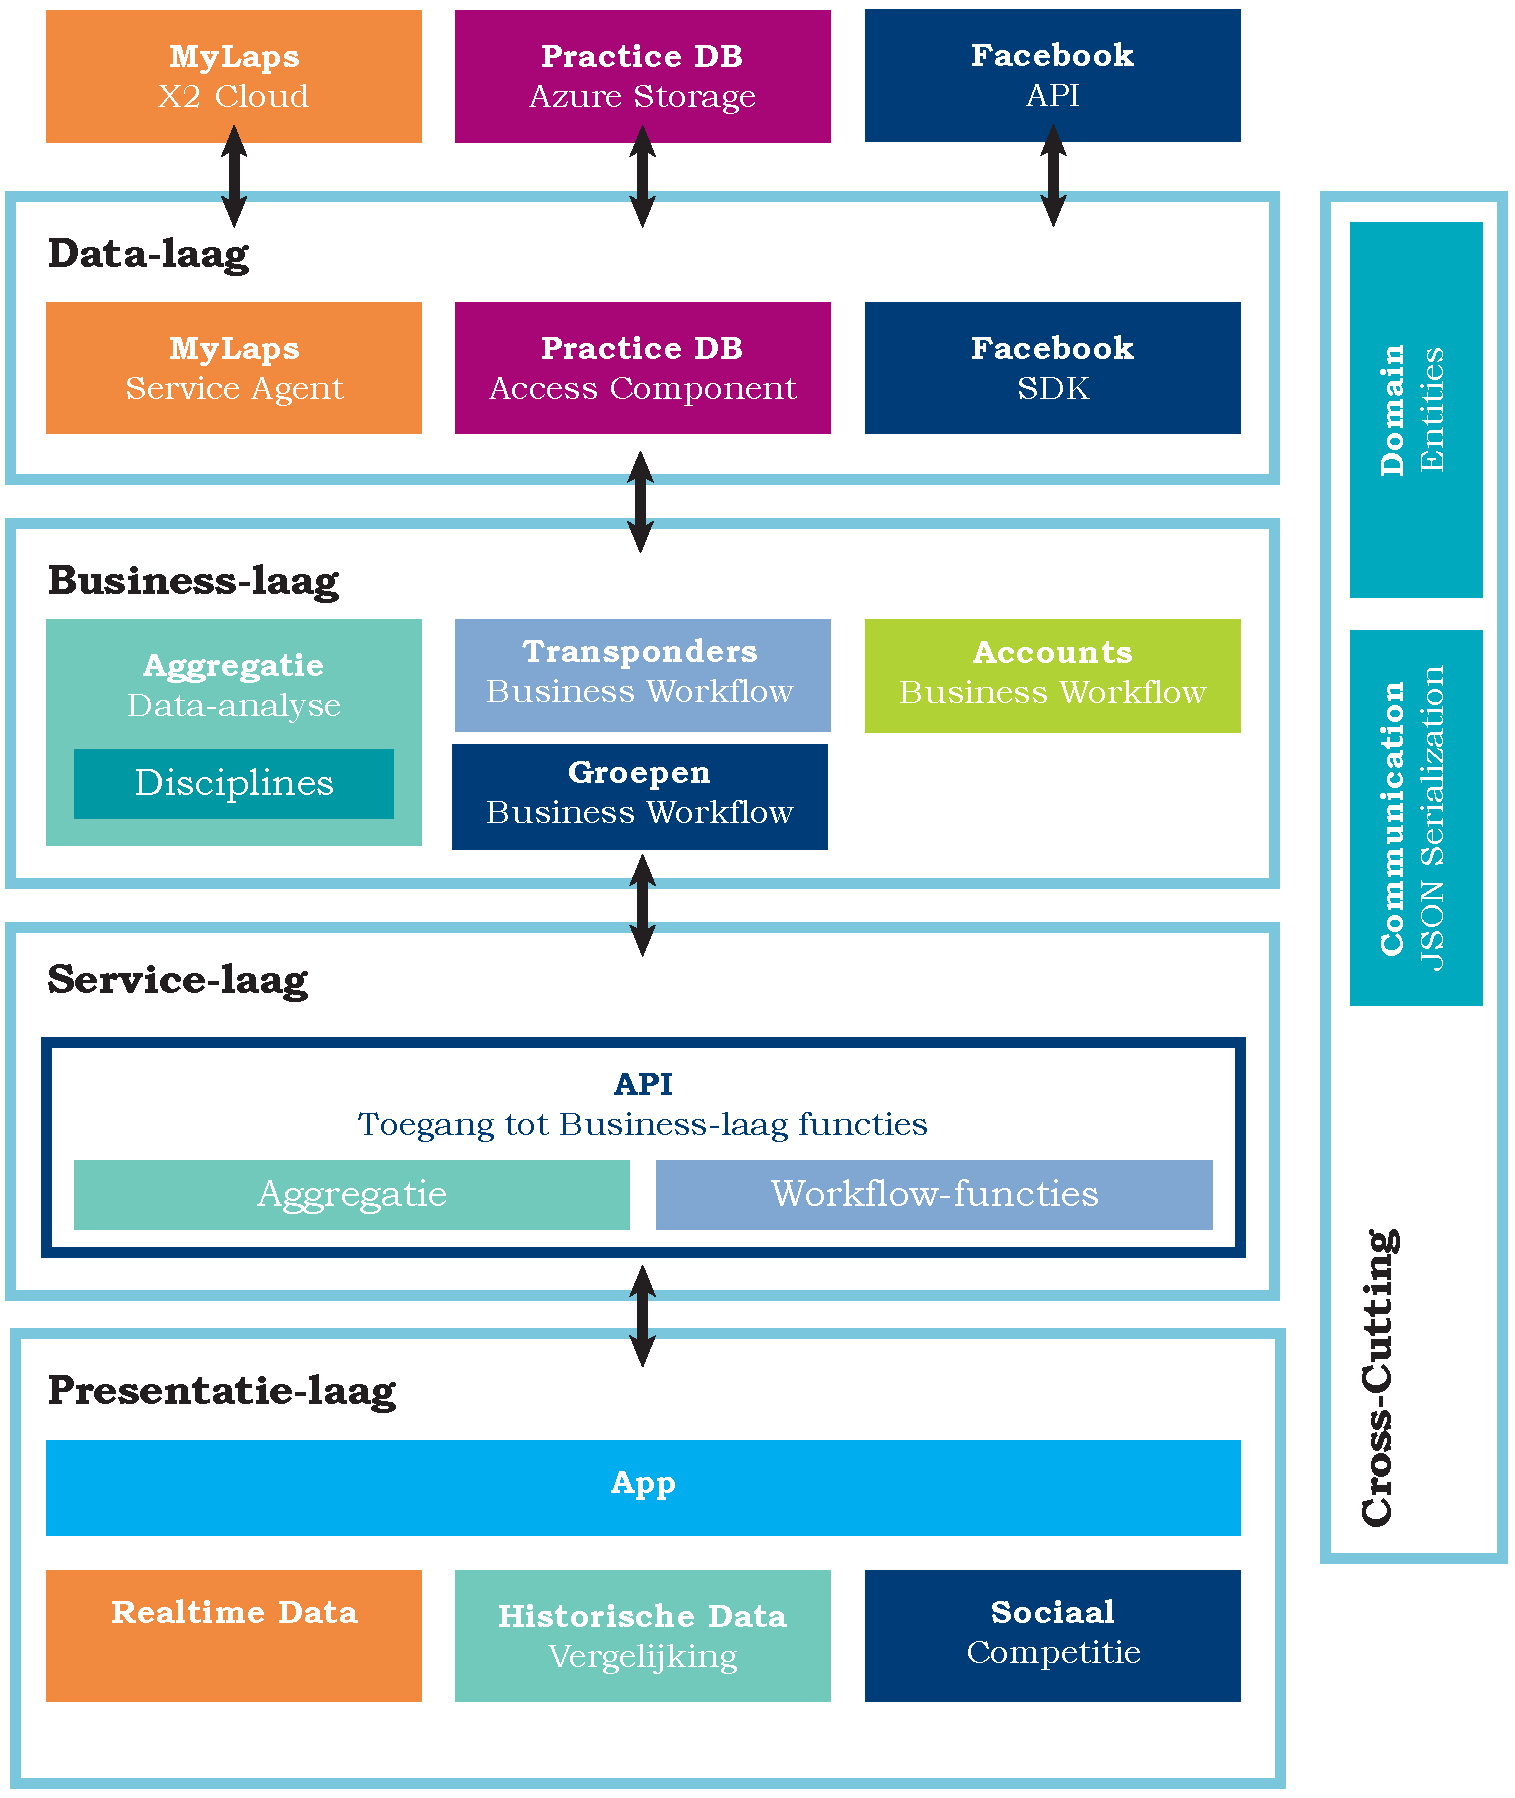
\includegraphics[width=0.6\textwidth]{style/images/Layers}
  \caption{Diagram van de lagen van de applicatie}
  \label{fig:diagram-layers}
\end{wrapfigure}

Zoals besproken tijdens de meeting van 23 april (Pagina \pageref{sec:meeting-23-apr}), worden applicaties die Emando ontwikkelt opgedeeld in vier lagen. Deze opzet zullen wij ook aanhouden.

\begin{description}
\item[De presentatielaag] verzorgt de weergave. De presentatielaag bevind zich in de code van de mobiele applicatie en bevat zowel platform onafhankelijke View-Models en hulpmiddelen als platform specifieke User Interface elementen.
\item[De servicelaag] is de interface tussen de server en de mobiele apps. Deze gebruikt de twee technieken SignalR en WebApi.
\item[De businesslaag] is verantwoordelijk voor het ophalen en verwerken van de data. Deze laag bevat een verbinding met de service- en datalaag. Met deze verbindingen is deze laag is staat met behulp van logica data op te halen, te verwerken, eventueel op te slaan en door te sturen naar de servicelaag. 
\item[De datalaag] is verantwoordelijk voor alle verschillende databronnen: Entity Framework, Table Storage en MyLaps. Deze laag bevat zelf geen verbindingen andere lagen, maar de data kan met behulp van repositories vanuit de business laag opgevraagd worden.

\end{description}

Naast deze vier lagen is er ook nog een deel van de code die gedeeld wordt door alle andere lagen: \textbf{``cross-cutting''}. In de cross-cutting laag bevinden zich voornamelijk de domein entiteiten, zodat alle server-lagen deze entiteiten kunnen gebruiken. Naast de entiteiten wordt ook de JSON serialisatie van de entiteiten in de cross-cutting laag geregeld: er zijn  speciale te serialiseren afgeleide modellen, met zo weinig afhankelijkheden van frameworks dat ze in een \ac{pcl} kunnen. Hierdoor kunnen de mobiele applicaties dezelfde modellen gebruiken als de servicelaag, en kunnen de modellen via de Websockets- en HTTP-verbinding van SignalR en WebAPI verstuurd worden. Deze entiteiten bevatten allen een context Id en user Id, welke aangeeft voor welke context (groep, baan of gebruiker) bedoelt is en van wie deze entiteit is. Op deze manier is SignalR in staat om deze entiteiten te versturen naar de juiste gebruikers.

  % 4 lagen
  % - presentatie laag
  % - service laag: API
  % - business laag: analyse en aggregatie
  % - data laag
  
\section{Datalaag}
De applicatie bevat data uit verschillende bronnen, en slaat zijn data in verschillende bronnen op. Deze data en de verbindingen met de bronnen vormen de datalaag.

\subsection{Ruwe inkomende data}

De transponderleverancier MYLAPS heeft een SDK beschikbaar gesteld aan Emando, waarmee het mogelijk is om de doorkomsten van transponders realtime binnen te krijgen. Om deze databron te benaderen bevat de datalaag een Data Collector, geïmplementeerd als Azure Cloud Worker Role, welke non-stop draait op één cloud instance. Dit proces onderhoudt de verbinding met de MYLAPS SDK.

Vanuit de MyLAPS SDK ontvangt de data laag realtime de doorkomsten van iedere transponder die langs een lus komt. Deze doorkomsten bevatten een tijdstip, een transponder nummer en een plaats op de baan. Zodra een van deze doorkomsten binnen komt, wordt deze direct opgeslagen voor toekomstig gebruik in een doorkomsten tabel in Azure Table Storage. Het kan namelijk voorkomen dat er op dit moment geen gebruiker van onze applicatie is, welke zijn transponder nummer heeft gekoppeld aan zijn account. Wanneer dit het geval is, kunnen er (nog) geen aggregaties uitgevoerd worden op deze data.

\begin{figure}[ht]
  \begin{center}
  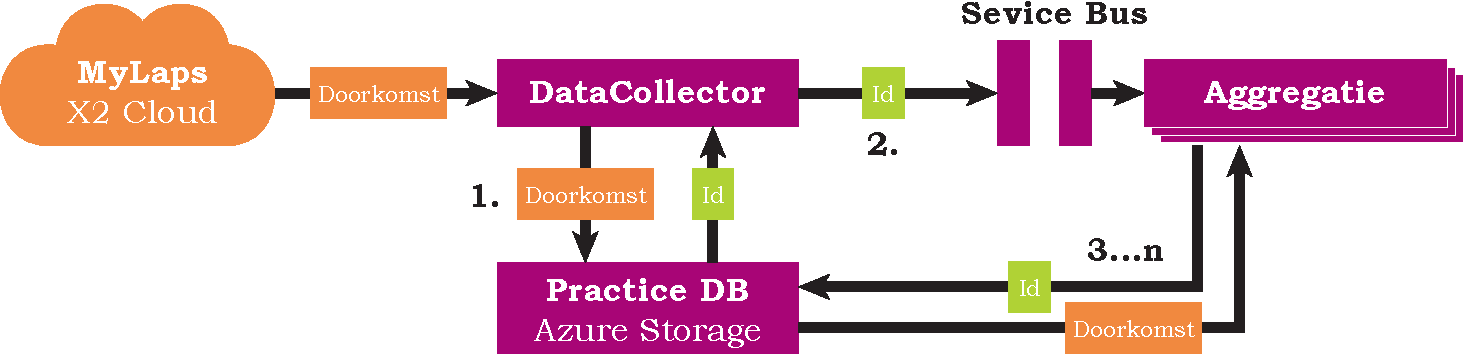
\includegraphics[width=\textwidth]{style/images/datacollector-flow}    
  \end{center}
  \caption{De werking van de Data Collector en de Service Bus}
  \label{fig:datacollector}
\end{figure}

Door deze data op te slaan, is het mogelijk om later functionaliteit in te bouwen om alsnog over deze data te kunnen aggregeren.

Nadat de data opgeslagen is, wordt via een Azure Service Bus het Id van de doorkomst doorgestuurt naar het aggregatie process in de businesslaag. Het aggregatie process raadpleegt bij het binnenkrijgen van dit Id opnieuw de doorkomst, om zo minder data over de service bus te versturen en altijd over up to date data te beschikken. Dit process wordt weergegeven in figuur~\ref{fig:datacollector}.

\subsection{Entiteiten}
In Figuur~\ref{fig:entiteiten} wordt een deel van de entiteiten die de applicatie gebruikt getoond, inclusief de onderlinge relaties. De entiteiten die te maken hebben met {\bfseries\color{tudelft-dark-blue} externe data} en {\bfseries\color{tudelft-green} accounts} worden opgeslagen met behulp van Azure SQL, zoals ook besproken in sectie~\ref{sec:database} van het oriëntatieverslag. De entiteiten die te maken hebben met {\bfseries\color{tudelft-orange} passings} en {\bfseries\color{tudelft-warm-purple} aggregaties} worden opgeslagen in Azure Table Storage.

\begin{figure}[ht]
  \begin{center}
  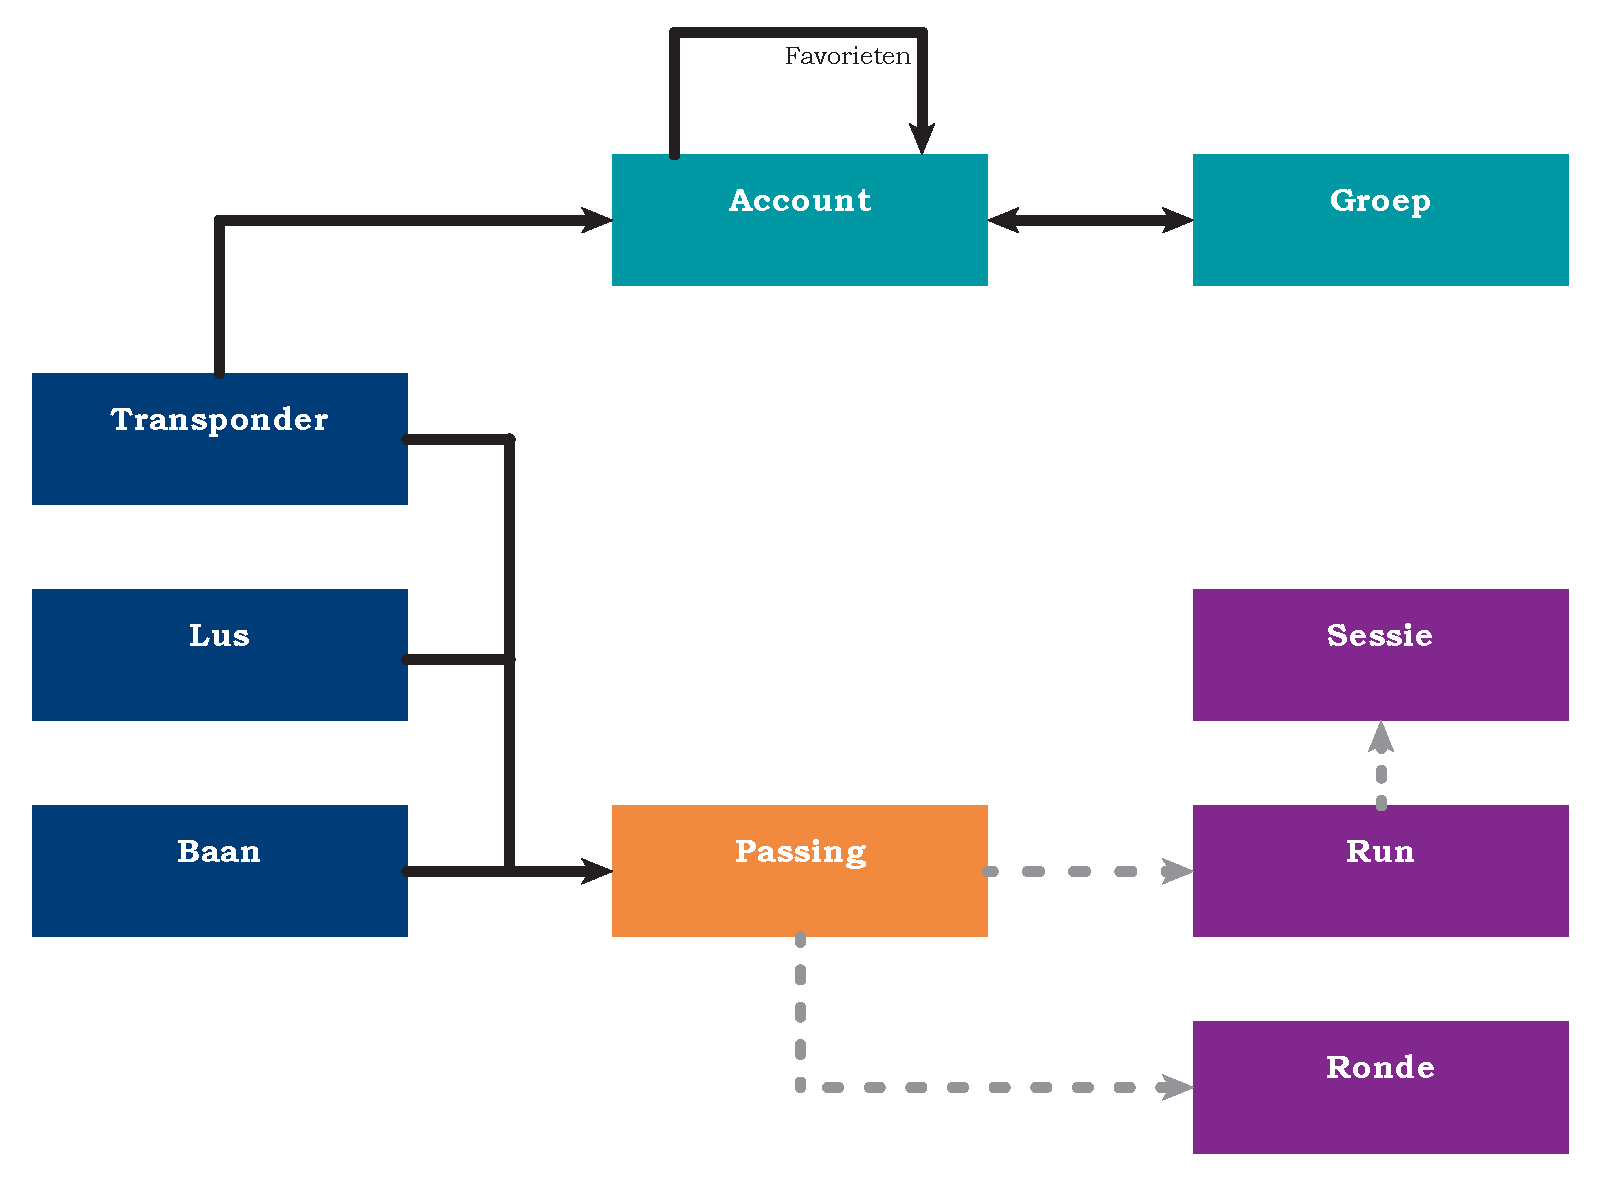
\includegraphics[width=.6\textwidth]{style/images/Entiteiten}    
  \end{center}
  \caption{De entiteiten en hun relaties.}
  \label{fig:entiteiten}
\end{figure}

Hoewel de daadwerkelijke structuur van de data in Azure Table Storage anders is dan in de figuur, geeft de figuur toch een goed beeld van deze entiteiten en hun relaties. 

\subsection{Azure SQL \& Entity Framework}
Azure SQL is de relationele SQL database van Azure en omdat de relaties in onze entiteiten worden beschreven door het Entity Framework~\cite{entityframework-msdn, entityframework-facto}, gebruikt onze applicatie de Entity Framework driver voor Azure SQL. Entity Framework is de defacto standaard voor relationele datalagen in ASP.NET. Het kan bijvoorbeeld relaties tussen entiteiten automatisch opzoeken. Ook hoeft er geen SQL code geschreven te worden, maar kan platformonafhankelijke LINQ code geschreven worden om entiteiten op te halen.

\subsection{Azure Table Storage}
De geaggregeerde data kan plat worden opgeslagen met behulp van NoSQL. Dit komt doordat alleen passings (doorkomsten), rondes en leaderboard-waarden entiteiten zijn in de aggregatie database. Zowel de sessie als het zijn van run of dan wel rust zijn eigenschappen van een ronde. De snelheid en segmenten worden niet opgeslagen.

Vanuit Emando ging de voorkeur voor het opslaan van de geaggregeerde data  uit naar de NoSQL Azure Table Storage. De Table Storage integreert eenvoudig met de reeds bestaande infrastructuur van het bedrijf. Bovendien biedt een gepartitioneerde en gesorteerde Table Storage tabel een groot performance voordeel: het goedkoop en snel kunnen selecteren van de laatste entiteiten per context.

Vanuit de Data Collector worden de doorkomsten die realtime binnen komen opgeslagen in Table Storage als backup. De structuur van deze tabel is terug te vinden in {\color{red} ref en tabel toevoegen }. Verderop in het aggregatieproces worden deze doorkomsten gekoppeld aan gebruikers. Deze aggregaties worden vervolgens opgeslagen in een aparte tabel binnen Azure Table Storage. De structuur van deze tabel is terug te vinden in {\color{red} ref en tabel toevoegen }.

Van snelheden, rondes, run/rust periodes en sessies worden leaderboards bijgehouden in Azure Table Storage. Deze hebben allen een eigen corresponderende tabel, zodat aggregaties parallel aan elkaar leaderboards kunnen updaten {\color{red} ref aggregatielaag }.
Alle leaderboards zijn voorzien van een leaderboard Id en een user Id. Het leaderboard Id houdt bij voor welke context het leaderboard geldig is. Dit kunnen banen, groepen, maar ook gebruikers zijn. Wanneer een gebruiker een ronde rijdt op een baan X, moeten zijn records voor de baan, zijn groepen en zijn eigen totalen geüpdatet worden. 

\begin{figure}[ht]
  \begin{center}
  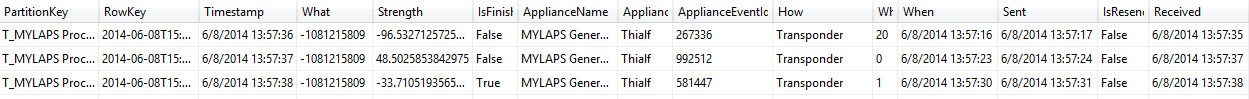
\includegraphics[width=.6\textwidth]{style/images/passingsStructure}    
  \end{center}
  \caption{De doorkomsten tabel met voorbeeld records. Hierbij is de Partition Key het type trasponder + transponder nummer en de Row Key het tijdstip waarop de doorkomst binnen kwam.}
  \label{fig:passingTableStructure}
\end{figure}

\begin{figure}[ht]
  \begin{center}
  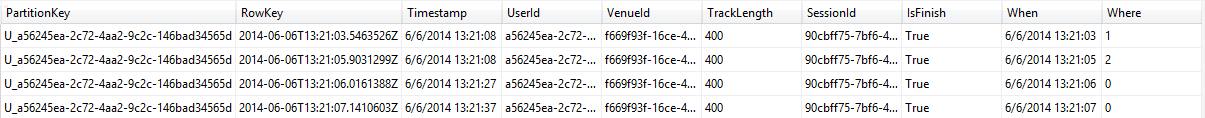
\includegraphics[width=.6\textwidth]{style/images/userPassingsStructure}    
  \end{center}
  \caption{De doorkomsten tabel met voorbeeld records. Hierbij is de Partition Key het account Id met een prefix voor gebruikers en de Row Key het tijdstip waarop de doorkomst binnen kwam.}
  \label{fig:userPassingTableStructure}
\end{figure}

\begin{figure}[ht]
  \begin{center}
  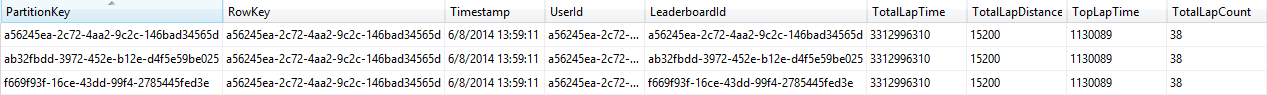
\includegraphics[width=.6\textwidth]{style/images/lapLeaderboardStructure}    
  \end{center}
  \caption{De ronde tabel met voorbeeld records. Hierbij is de Partition Key het account Id en de Row Key het ronde Id.}
  \label{fig:lapTableStructure}
\end{figure}

\begin{figure}[ht]
  \begin{center}
  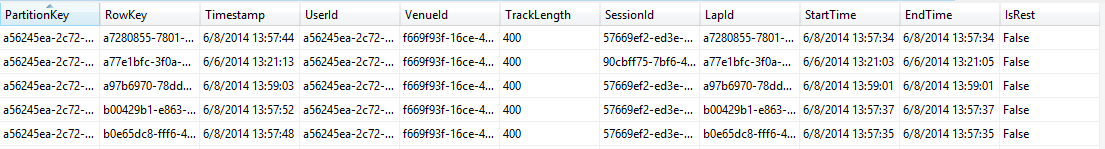
\includegraphics[width=.6\textwidth]{style/images/aggregationLapsStructure}    
  \end{center}
  \caption{De ronde leaderboard tabel, een voorbeeld van een leaderboard tabel. Hierbij is de Partition Key het account Id en de Row Key het context Id (groep, baan of account Id).}
  \label{fig:entiteiten}
\end{figure}

De structuur van de leaderboard tabellen ziet er als volgt uit.
{\color{red} tabel toevoegen}
\section{Businesslaag}
  De businesslaag bestaat uit meerdere grote onderdelen. Zowel aggregatie als de workflows zijn twee gescheiden onderdelen die zich in de businesslaag bevinden.
 
\begin{figure}[ht]
  \begin{center}
  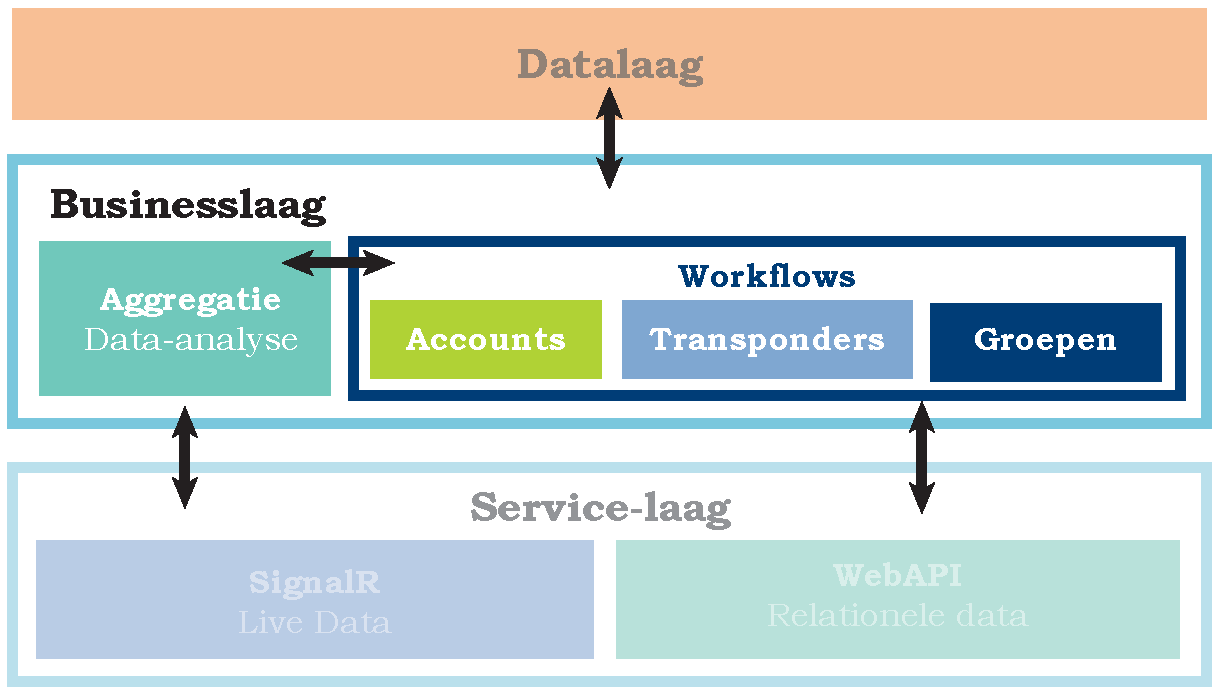
\includegraphics[width=.6\textwidth]{style/images/Businesslaag}    
  \end{center}
  \caption{Opbouw en interactie van de businesslaag}  
  \label{fig:lagen-businesslaag}
\end{figure}
  
  
  De businesslaag is de plek waar de communicatie met de datalaag en de servicelaag plaats vindt. Vanwege de keuze om de data realtime door te geven aan de applicatie is het belangrijk dat deze laag snel en vloeiend werkt, ook bij een hoge load. Om deze reden hebben we gekozen voor een Cloud-oplossing in Windows Azure, welke draait op een of meerdere Cloud instances. Bij een hogere load worden er automatisch voldoende extra instances aangemaakt en wordt de load evenwichtig verdeeld. Tevens biedt een Cloud-oplossing de mogelijkheid om verbeteringen aan bestaande of juist nieuwe functionaliteit toe te voegen aan de back-end, zonder dat de applicatie hierbij een update vereist.

Hoewel er meerdere soortgelijke Cloud-oplossingen bestaan, ging vanwege de bestaande infrastructuur van Emando de voorkeur uit naar Windows Azure. Een bijkomend voordeel van Windows Azure is de eenvoudige integratie met Visual Studio, waardoor het deployen naar de cloud- of testomgeving gemakkelijk is.

\subsection{Aggregatiestructuur}

Omdat de ruwe doorkomsten niet direct betekenis hebben voor gebruikers, dient deze data verrijkt te worden om zo inzicht te geven in trainingen van gebruikers. Dit proces noemen we de aggregatie van data.

Zodra er een doorkomst binnenkomt binnen de datalaag, wordt het Id hiervan naar de aggregatielaag overgestuurd via de Azure Service Bus. Zodra de aggregatielaag deze ontvangt, wordt de bijbehorende doorkomst opgevraagd. Hierna start het aggregatieproces, dat bestaat uit de volgende onderdelen, zoals ook te zien is in figuur~\ref{fig:aggregatie-flow}:

\begin{itemize}
\item \textbf{Reguliere filters.}
Deze filters vergelijken reeds bestaande geaggregeerde en ruwe data met de nieuwste binnenkomst, om zo nieuwe data te aggregeren. Deze data wordt vervolgens doorgegeven aan de dispatchers en top filters. Voorbeeld: Het opmaken van rondetijden aan de hand van verschillende doorkomsten op een baan.
\item \textbf{Top filters.}
Deze filters vergelijken reeds bestaande geaggregeerde data met de zojuist geaggregeerde data, om zo te kijken of de zojuist geaggregeerde data een record bevat voor de gebruiker. Deze filters verwerken de nieuwe records in de leaderboards voor een gebruiker op gebruikers-, baan- en groepsniveau. Vervolgens worden deze leaderboards doorgegeven aan de dispatchers. Voorbeeld: Een gebruiker heeft een nieuwe ronde geschaatst, waarin zijn rondetijd verbeterd is, maar ook zijn totale afstand op de baan toegenomen is. 
\item \textbf{Dispatchers.}
De dispatchers ontvangen alle geaggregeerde data en zijn verantwoordelijk voor het doorgeven van deze data aan de juiste applicaties. De dispatchers zorgen er voor dat deze data realtime binnen komt bij alle geïnteresseerden van deze updates. 
Voorbeeld: Live doorkomsten van gebruikers van een groep/baan. 
\end{itemize}

De filters zijn opgebouwd volgens een pipeline-structuur. Na het uitvoeren van een filter worden de filters aangeroepen die de filteruitvoer als invoer verwachten. Als een filter geen aggregatie uit kan voeren, stopt de aggregatie bij dit filter, aangezien er zonder de uitvoer van dit filter, geen andere filters aangeroepen kunnen worden. 

\begin{figure}[h]
  \begin{center}
    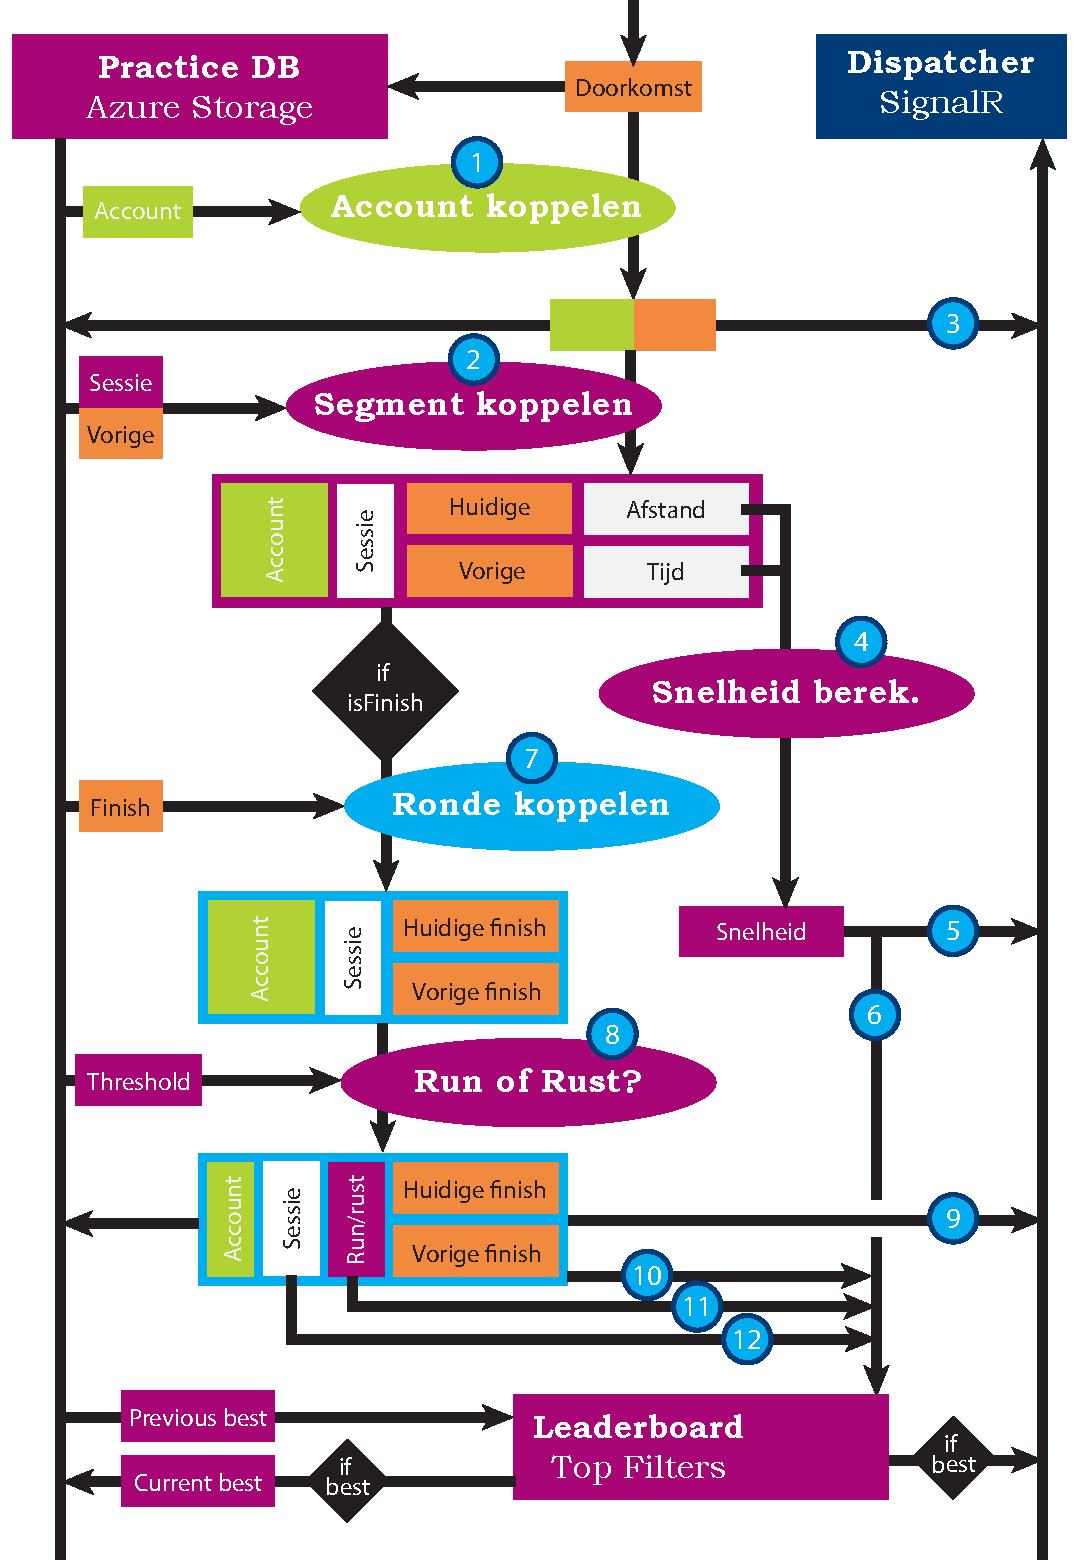
\includegraphics[width=.4\textwidth]{style/images/Aggregatie-flow}
  \end{center}
  \caption{Flow-diagram van het aggregatieproces \\ N.B. Deze afbeelding is in groot formaat opgenomen in Appendix~\ref{ch:aggregation-flow} op pagina~\pageref{fig:aggregatie-flow-large}.}
  \label{fig:aggregatie-flow}
\end{figure}

\begin{enumerate}

\item \textbf{Account koppelen aan doorkomsten.}

Allereerst wordt bij een doorkomst aan de hand van het transponder nummer een account gezocht. Als er een bestaande gebruiker is die dit transpondernummer momenteel aan zijn account gekoppeld heeft, wordt dit account gekoppeld aan deze doorkomst. Dit wordt opgeslagen in een aparte tabel in Azure Table Storage.

\item \textbf{Doorkomsten koppelen aan segmenten.}
Een doorkomst maakt deel uit van een training, soms gekoppeld aan een trainingsschema. Een training kan bestaan uit een of meerdere sessies. Een segment van doorkomsten houdt in dat er twee doorkomsten van dezelfde gebruiker binnen 30 minuten hebben plaatsgevonden op dezelfde baan. Wanneer de vorige doorkomst van deze gebruiker en de huidige doorkomst binnen een segment vallen, vallen deze doorkomsten onder dezelfde trainingssessie. Wanneer dit het geval is, krijgt de doorkomst dezelfde sessie Id toegewezen als zijn vorige doorkomst. Wanneer dit niet het geval is of wanneer er geen vorige doorkomst is, kan er geen segment gevonden worden.

\item \textbf{Dispatchen van live doorkomsten.}
Zodra er een gebruiker gevonden is bij een doorkomst, moet deze doorgegeven worden aan alle ``geïnteresseerden'': de gebruiker zelf, gebruikers op dezelfde baan, leden van dezelfde groep als deze gebruiker en alle gebruikers die geabonneerd zijn op deze gebruiker.

Met behulp van SignalR wordt de doorkomst doorgegeven aan de juiste personen.

\item \textbf{Snelheid berekenen.}
Tussen twee doorkomsten in een segment ligt een bepaalde afstand. Een gebruiker heeft deze afstand afgelegd in een tijdsinterval. Aan de hand van deze gegevens wordt de snelheid binnen dit segment berekend.

\item \textbf{Dispatchen van snelheden.}
Zodra er een snelheid is berekend voor een gebruiker op een bepaald segment, moet deze doorgegeven worden aan alle eerder genoemde geïnteresseerden.

Met behulp van SignalR wordt de doorkomst doorgegeven aan de juiste personen.

\item \textbf{Snelheidsleaderboard updaten en dispatchen.}
Zodra er een snelheid berekend is over een bepaald segment, kan dit gevolgen hebben voor het snelheidsleaderboard. De gereden snelheid wordt vergeleken met de eerdere persoonlijke records van de gebruiker, zijn records op deze baan en zijn records in al zijn groepen. Daarnaast wordt altijd de gereden afstand op de baan, tijdsinterval etc. bijgewerkt in de totalen binnen dit leaderboard. Wanneer de zojuist gereden snelheid een record blijkt te zijn voor een van zojuist genoemde contexten, wordt deze up to date gebracht in de leaderboards. Daarna wordt het gehele leaderboard voor deze context via SignalR naar alle geïnteresseerden verstuurd.

\item \textbf{Doorkomsten koppelen aan rondes.}
De gevonden sessie bij het segment kan gebruikt worden om rondes te vinden. Wanneer de huidige doorkomst afkomstig is van de finish-lus en de gebruiker in de huidige sessie een eerdere doorkomst op de finish-lus heeft, is er sprake van een ronde in een training. 
Wanneer de sessie Ids niet overeenkomen, of de huidige doorkomst niet op de finish lijn ligt is het niet mogelijk om een ronde te vinden.

\item \textbf{Filteren van run- en rustperiodes.}
Afhankelijk van het type sporter, wordt er al dan niet getraind aan de hand van een trainingsschema. Deze schema's bestaan vaak uit run- en rustperiodes waarin respectievelijk hard getraind wordt of langzaam wordt uitgereden. Omdat de lengte van rondes kan variëren op verschillende banen, wordt niet aan de hand van tijden, maar snelheden gefilterd. Wanneer de gemiddelde snelheid in een ronde hoger is dan een vooraf ingestelde snelheid, wordt deze ronde beschouwd als een run-ronde. Anders wordt deze beschouwd als onderdeel van een rustperiode. Nu alle ronde data compleet is, wordt deze ronde opgeslagen in een aparte tabel in Azure Table Storage voor latere aggregaties.

\item \textbf{Dispatchen van rondes.}
Zodra er een ronde is berekend voor een gebruiker, wordt deze opnieuw met behulp van SignalR naar de eerder genoemde geïnteresseerden verstuurd.

\item \textbf{Rondeleaderboard updaten en dispatchen.}
Zodra er een ronde is gevonden voor een gebruiker, kan dit gevolgen hebben voor het rondeleaderboard. De gereden ronde wordt vergeleken met de persoonlijke records voor een gebruiker, zijn records op deze baan en zijn records in al zijn groepen. Daarnaast wordt altijd de gereden afstand op de baan, tijdsinterval etc. bijgewerkt in de totalen binnen dit leaderboard. Wanneer de zojuist gereden rondetijd een record blijkt te zijn voor een van zojuist genoemde contexten, wordt deze up to date gebracht in de leaderboards. Daarna wordt het gehele leaderboard voor deze context naar alle geïnteresseerden gestuurd via SignalR.

\item \textbf{Run/rustleaderboard updaten en dispatchen.}
Zodra er een ronde is gevonden voor een gebruiker, kan dit gevolgen hebben voor het run/rustleaderboard. De gereden rondetijd wordt toegevoegd aan de desbetreffende run/rustperiode en aan de hand hiervan wordt het totaal hiervan vergeleken met de persoonlijke records voor een gebruiker, zijn records op deze baan en zijn records in al zijn groepen. Daarnaast wordt altijd de gereden afstand op de baan, tijdsinterval etc. bijgewerkt in de totalen binnen dit leaderboard. Wanneer de zojuist gereden rondetijd een record blijkt te zijn voor een van zojuist genoemde contexten, wordt deze up to date gebracht in de leaderboards. Daarna wordt het gehele leaderboard voor deze context naar alle geïnteresseerden gestuurd via SignalR.

\item \textbf{Sessie leaderboard updaten en dispatchen.}
Zodra er een ronde is gevonden voor een gebruiker, kan dit gevolgen hebben voor het sessie leaderboard. De gereden rondetijd wordt toegevoegd aan de desbetreffende sessie en aan de hand hiervan wordt het totaal hiervan vergeleken met de persoonlijke records voor een gebruiker, zijn records op deze baan en zijn records in al zijn groepen. Daarnaast wordt altijd de gereden afstand op de baan, tijdsinterval etc. bijgewerkt in de totalen binnen dit leaderboard. Wanneer de zojuist gereden rondetijd een record blijkt te zijn voor een van zojuist genoemde contexten, wordt deze up to date gebracht in de leaderboards. Daarna wordt het gehele leaderboard voor deze context naar alle geïnteresseerden gestuurd via SignalR.

\end{enumerate}

\subsection{Dataconsistentie en parallellisering}
Vanwege de meeschalende Cloud-oplossing, kan het voorkomen dat aggregaties van één persoon over meerdere instances berekend worden. Het is belangrijk dat deze aggregaties parallel lopen om gebruikers van realtime updates te kunnen voorzien. Dit brengt echter wel het probleem met zich mee dat sommige data afhankelijk is van andere data en dat deze data consistent moet blijven met elkaar. De eerder genoemde pipeline-architectuur zorgt er voor dat bij ieder filter bekend is welke afhankelijkheden hierop berusten. Zodra het filter klaar is met zijn aggregatie, wordt gekeken of de aggregatie bruikbaar is voor zijn afhankelijkheden en geeft zijn aggregatie aan de hand hiervan door. Deze afhankelijkheden kunnen op hun beurt over verschillende instances verdeeld worden, zonder dat er opstoppingen ontstaan.

Omdat onze aggregatielaag berust op de \mylaps SDK en een service bus, kan het in theorie voorkomen dat een eerdere doorkomst pas later bij deze laag binnenkomt dan een latere doorkomst. Ook kan het voorkomen dat het berekenen van een aggregatie van een eerdere doorkomst langer duurt dan die van een latere doorkomst, waardoor de updates hiervan door elkaar heen gaan lopen. Dit is te zien in figuur~\ref{fig:aggregatie-timing-problem}. 
In deze figuur is te zien hoe doorkomst~3 later gereden wordt, maar eerder geaggregeerd wordt dan doorkomst~2 welke eerder gereden is. Doordat de aggregatie werkt met de vorige doorkomst (doorkomst~1) wordt doorkomst~3 gekoppeld aan doorkomst~1 in een segment waarover de snelheid berekend wordt. Hieruit komt een correcte waarde.

Wanneer doorkomst~2 echter geaggregeerd wordt, vraagt deze de vorige doorkomst op. Omdat doorkomst~3 al geaggregeerd was, is doorkomst~3 zijn vorige doorkomst. Hierbij wordt doorkomst~2 gekoppeld aan doorkomst~3. In dit segment blijkt nu -100 meter gereden te zijn. Er zou nu een verkeerde aggregatie ontstaan!

Daarom is het belangrijk dat de data te allen tijde consistent is, ook over meerdere Cloud instances.
Om deze reden zijn alle repositories calls voorzien van een synchronisatietijdstip. Dit is het tijdstip waarop de doorkomst doorgekomen is. Deze calls geven daarmee alleen (aggregatie)data terug die op het moment van de doorkomst beschikbaar was. In het bovengenoemde geval zou doorkomst~2 daarom óók gekoppeld worden aan doorkomst~1, vanwege het feit dat doorkomst~3 later binnen gekomen is dan doorkomst~2. Op deze manier worden inconsistenties in de data voorkomen.

\begin{figure}[ht]
  \begin{center}
    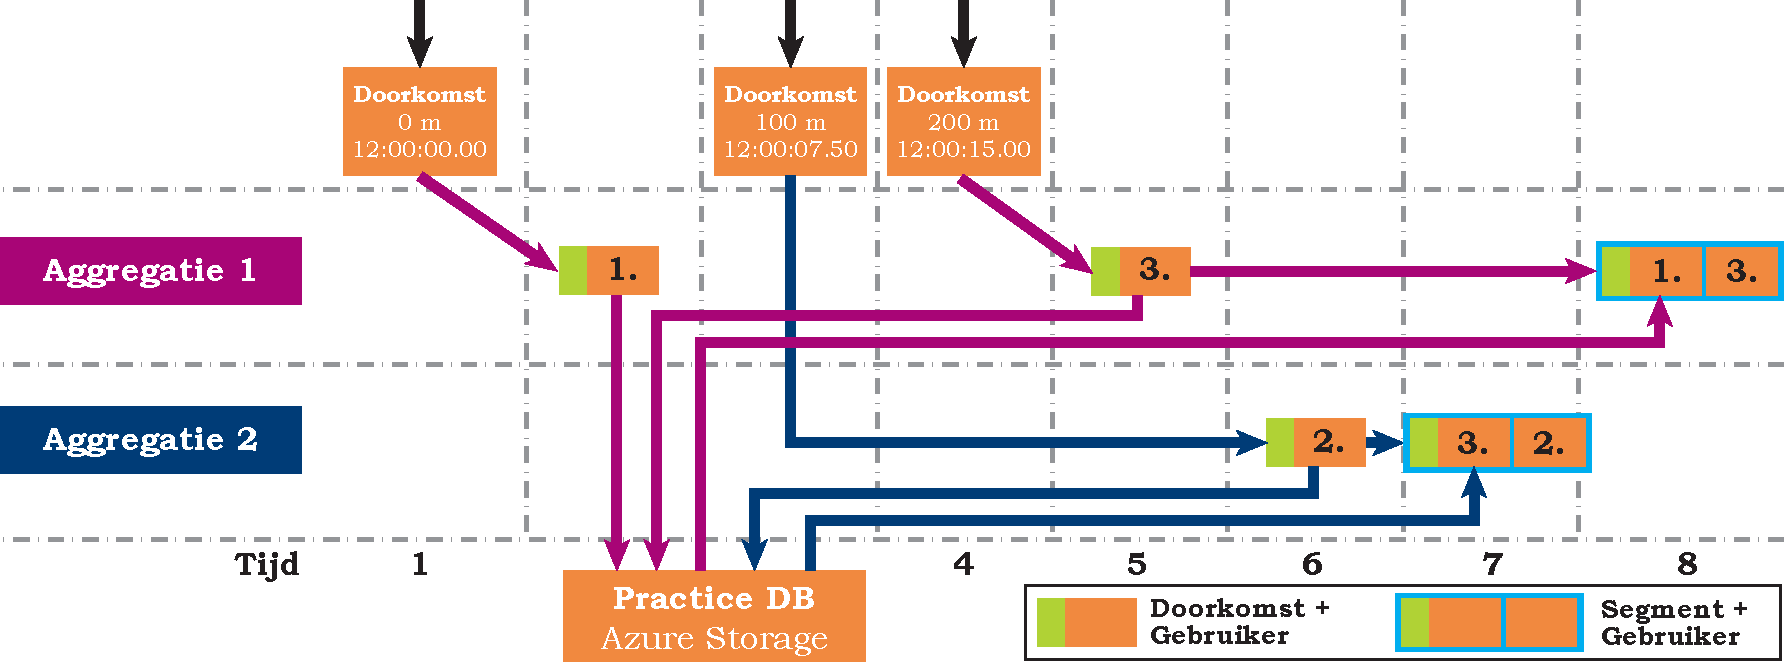
\includegraphics[width=\textwidth]{style/images/aggregatie-timing-problem}
  \end{center}
  \caption{Flow-diagram van hoe de data stroom verkeerd kan gaan.}
  \label{fig:aggregatie-timing-problem}
\end{figure}

Voor de leaderboards is gekozen om deze te verspreiden over vier aparte tabellen. Leaderboards bestaan uit data die vanuit verschillende filters aangepast worden. Hierbij wordt eerst het leaderboard opgevraagd en daarna de update teruggeschreven naar de tabel. Bij het updaten is het mogelijk om een merge-operatie uit te voeren, waarbij alleen de beschikbare data (bijvoorbeeld een snelheidsleaderboard) bij te werken zonder daarbij de bestaande data aan te passen. Dit kan echter alleen wanneer de ETag-eigenschap van dit leaderboard ondertussen niet gewijzigd is. Deze ETag-eigenschap is een onderdeel van Azure Table Storage dat bijhoudt of het record in de tussentijd al dan niet gewijzigd is. In de praktijk komen tussentijdse wijzigingen vaak voor, doordat er meerdere filters parallel aan elkaar hetzelfde record bij proberen te werken voor andere leaderboard eigenschappen. Om deze reden is beter om de leaderboards te spreiden over meerdere tabellen.


  \subsection{Workflows}

Een onderdeel van de Businesslaag zijn de workflows. Workflows zijn afgebakende taken, 
welke door de eenvoudig door de servicelaag en andere businesslaagprocessen zijn aan te roepen, 
en waarbij de servicelaag niet hoeft te weten hoe de taken worden uitgevoerd, 
als er maar het beoogde resultaat oplevert. In onze applicatie zijn er op 3 gebieden workflows, zoals ook te zien is in figuur~\ref{fig:lagen-businesslaag}:

\begin{itemize}
	\item{\textbf{Gebruikersaccounts beheren.}} 
	De AccountWorkflow biedt mogelijkheden om accounts aan te maken met zowel gebruikersnaam en wachtwoord als met een Facebook authenticatie sleutel (``access token''). Verder kunnen accounts worden opgezocht aan de hand van hun emailadres of unieke nummer. De servicelaag biedt deze workflow rechtstreeks aan via de API.

	\item{\textbf{Transponders beheren.}} 
	Gebruikers kunnen per tijdseenheid maar één transponder hebben en deze kan niet door meer mensen tegelijk geregisteerd zijn. Deze logica wordt verzorgt voor de servicelaag, zodat gebruikers transponders kunnen toevoegen en kunnen ontkoppelen van hun account en daar de juiste eventuele foutmeldingen bij krijgen. Daarnaast moet de businesslaag snel kunnen opzoeken welke gebruiker bij een transponder hoort, op het moment dat een doorkomst binnenkomt. De TransponderWorkflow bevat de logica ervoor om deze checks te doen en de transponders op te zoeken.

	\item{\textbf{Groepen beheren.}} 
	Het aanmaken en beheren van groepen zijn ook specifieke taken waar een GroupWorkflow voor bestaat. Deze workflow zorgt er voor dat de actieve gebruiker wordt toegevoegd aan de aangemaakte groep en dat er alleen wijzigingen plaatsvinden die mogen worden uitgevoerd. Deze logica voornamelijk door de servicelaag gebruikt, om de groepen functionaliteit aan te bieden. Daarnaast wordt beschikbare nieuwe informatie doorgestuurd naar de gebruikers uit dezelfde groepen. Ook hiervoor wordt de workflow gebruikt.

\end{itemize}
  
\section{Servicelaag}
  Onze applicatie bevat data met verschillende relevantie over tijd. Tijdens het sporten zijn vooral doorkomsten interessant evenals informatie over de actuele training. Ná het sporten zijn vergelijkingen met andere sporters interessant en analyses op de training. Zowel SignalR\footnote{\url{http://www.asp.net/signalr}} als WebApi\footnote{\url{http://www.asp.net/web-api}} zijn technieken om data door te sturen, maar SignalR is gemaakt voor live data en WebApi voor het toegankelijk maken van al bestaande data via een REST API~\footnote{\url{http://en.wikipedia.org/wiki/Representational_state_transfer}}. In onze applicatie gebruiken we dan ook beide technieken naast elkaar. Een derde techniek die we gebruiken is OWIN~\footnote{\url{http://www.asp.net/aspnet/overview/owin-and-katana}}, een brug tussen de webserver en de web-applicatie. OWIN verzorgt het opstarten en configureren van de web-applicatie.

\subsection{SignalR}
SignalR onderhoudt een continue verbinding tussen server en client waarbij het zelf zorgt voor het juiste onderliggende protocol. SignalR werkt bij voorkeur over WebSockets, maar werkt ook met oudere browsers door gebruik te maken van "polling". Bij polling houdt de server de verbinding zolang mogelijk open. Als er een bericht afgeleverd moet worden wordt deze verstuurd, de verbinding wordt gesloten, en er wordt weer een nieuwe verbinding gemaakt. Door gebruik te maken van SignalR hoeven we ons niet bezig te houden met de werking van deze ingewikkelde protocollen, en kunnen we eenvoudig een verbinding opzetten.

Naast het beheren van de individuele verbindingen, onderhoudt SignalR ook virtuele groepen. Een nieuw bericht kan gestuurd worden naar individuele gebruikers, maar ook naar deze groepen. Wij gebruiken de groepen als interesse-context: in onze applicatie kunnen gebruikers een scherm open hebben van een baan of een (vrienden)groep, ze zijn dan geïnteresseerd in de updates van alle gebruikers in die context. Wanneer één van de leden van de context aan het schaatsen is, en er moet een update gestuurd worden, dan sturen we met één commando aan iedereen die in die context een update.

\subsection{WebApi}
De API die we gemaakt hebben met WebApi 2.0 ontsluit data die niet ``live'' is. Onder andere de registratie en het ophalen van profieldata, groepen, favorieten en banen gebeuren via WebApi. WebApi heeft als voordeel dat het te gebruiken is zónder een SignalR client en ook dat het makkelijker te debuggen is dan SignalR, omdat er geen  websocketverbinding gemaakt hoeft te worden. Door een API aan te bieden kan ons platform in de toekomst ook gemakkelijk gebruik worden voor andere applicaties.

\subsection{OWIN}
Zowel SignalR als WebApi zijn als 'middleware' geconfigureerd in het opstartscript van OWIN. OWIN zorgt er voor dat een binnenkomend verzoek wordt afgehandeld door die middleware die het verzoek kan afhandelen. Zo worden verzoeken naar de api doorgestuurd naar WebApi en verzoeken naar de url /signalr worden doorgestuurd naar SignalR. 

In OWIN hebben we ook OAuth geconfigureerd. OAuth is een authenticatiestandaard waarbij een gebruiker kan inloggen met zijn gebruikersnaam en wachtwoord of via een externe dienst zoals Facebook. De client krijgt dan een "token", een sleutel, die meegestuurd moet worden met opvolgende verzoeken. Hiermee is de authenticatie centraal geregeld, want zowel SignalR als WebApi kunnen hier mee overweg.
  \subsection{Platform-onafhankelijke client}
Om in de mobiele applicatie de data van zowel SignalR als WebApi te ontsluiten is er een platform-onafhankelijke client gemaakt. Deze client bevat alle interactie met SignalR en WebApi zodat andere delen van de applicaties geen verbinding hoeven op te zetten en te onderhouden.

De client bevat dus methodes voor zaken als inloggen en registreren, welke zijn aangesloten op WebApi. Deze methodes zijn asynchroon en retourneren taken. Met de asynchrone taalelementen van C\#\footnote{\url{http://msdn.microsoft.com/en-us/library/hh191443.aspx}} kunnen eenvoudig de functies worden aangeroepen vanuit knoppen in de applicatie en worden taken afgewacht, zodat óf de voortgangs-indicator kan worden verborgen óf een foutmelding getoond kan worden.

De data die vanuit SignalR binnenkomt wordt als ``Observable'' weergegeven. Observables zijn taalelementen van C\# uit \ac{rx} en kunnen worden gezien als objecten die functies uitvoeren als er nieuwe data binnenkomt, door een functie te ``subscriben'' op een Observable. De data vanuit SignalR heeft het karakter van bijvoorbeeld \textit{de actuele snelheid van gebruiker X}. De Observable heet dan CurrentSpeed en een voorbeeld van een functie is er een die de snelheid op het telefoonscherm aanpast aan de net binnengekomen snelheid.

\subsection{Lokale opslag met Akavache}
Mobiele applicaties moeten anders omgaan met data dan desktop-applicaties in die zin dat mobiele applicaties elk moment gesloten kunnen worden. Telefoons hebben een beperkte hoeveelheid geheugen, en als het OS van de telefoon detecteert dat er te weinig geheugen vrij is kan een niet zichtbare applicatie abrupt worden afgesloten. Als een gebruiker onze applicatie even onderbreekt om een andere applicatie te bekijken dan kan de applicatie dus zomaar worden afgesloten. Om bij het terug komen in de applicatie na het afsluiten niet een leeg scherm te hoeven tonen, moeten we data opslaan op het permanente geheugen van de telefoon. Hiervoor gebruiken we Akavache\footnote{\url{https://github.com/akavache/Akavache}}.

Akavache is een library voor asynchrone en persitente key-value opslag voor C\# applicaties. Met Akavache is eenvoudig te checken of een model al geladen is, het eventueel nog te downloaden en dan op te vragen. 

Aangezien de ViewModels, die ook later nog aan bod komen in sectie ~\ref{sec:vm-reactive-ui}, niet opgeslagen kunnen worden (sommige eigenschappen kunnen niet worden geserialiseerd) moet er nog een vertaalslag plaatsvinden tussen de opgeslagen entiteiten en de ViewModels. Onze platform-onafhankelijke client doet dit voor alle entiteiten en zorgt er voor dat  de ViewModels in stand blijven gedurende de hele tijd dat de applicatie draait. Eventuele wijzigingen worden aangepast in de ViewModels, maar de ViewModels worden nooit vervangen.

\section{Presentatielaag}
  De presentatielaag bevind zich in de mobiele applicatie. Hieronder komen enkele karakteristieke onderdelen aan bod.
  \subsection{View Models en Reactive UI} 
\label{sec:vm-reactive-ui}

Voor de koppeling tussen views en data gebruiken we speciale ViewModels die een `lifetime' hebben die langer is dan de views die deze modellen gebruiken. Controllers vragen de ViewModels op en geven ze door aan de views. Elke view bind zich vast aan het ViewModel en als een veld van het model verandert, dan updaten de views automatisch. Dit werkt met ReactiveUI~\footnote{\url{http://www.reactiveui.net/}}, een UI framework dat gebruikmaakt van \ac{rx}. Elk veld van de ViewModels stuurt een notificatie naar alle luisterende views als het wordt aangepast. ReactiveUI levert hiervoor zowel het notificatie-systeem als het koppel systeem voor views. Een versimpeld voorbeeld is als volgt:

\begin{verbatim}
public class SpeedViewModel : ReactiveObject {
  private double _speed = 0;
  public double Speed { 
    get { return _speed; }
    set { RaiseAndSetIfChanged(ref _speed, value); }
  }
}

public class View : UIView, IViewFor<SpeedViewModel> {
  public View(SpeedViewModel model) {
    OneWayBind(
      model, vm => vm.Speed, 
      view => view.speedLabel.Text, 
      field => field.ToString("F") + " km/h"
    );
  }
}
\end{verbatim}
%\caption{Voorbeeld van ReactiveUI: een ViewModel en View}

Wanneer de controller nu een ViewModel aanpast, of er via SignalR een update binnenkomt, dan wordt de view direct aangepast. 

Naast het updaten van alleenstaande modellen, gebruiken we ook lijsten van modellen. Hiervoor gebruiken we ReactiveList's, uit ReactiveUI, welke notificaties kunnen sturen wanneer er een element wordt toegevoegd of wordt verwijderd uit de lijst. We updaten dan de bestaande tabel en hoeven niet de hele tabel opnieuw te tekenen.

Door gebruik te maken van ReactiveUI wordt het heel simpel om views te maken die `live' zijn en het zorgt er voor dat de code overzichtelijk blijft, omdat het invullen en updaten van de views met dezelfde code gebeurt en deze erg simpel is.

\subsection{Grafische user interface}

{\par \bigskip \par \color{red} TODO: Belachelijk veel screenshots toevoegen \par \bigskip \par }

De gebruikersinterface van de applicatie staat in principe los van de rest van de applicatie. Hoewel het grootste deel van de code gebruikt kan worden op verschillende platforms, moet de gebruikersinterface voor elk platform apart ontwikkeld worden. Tijdens dit bachelorproject is ervoor gelozen om alleen een specifieke gebruikersinterface te maken voor iPhones. Zoals eerder besproken, is hiervoor gekozen omdat het grootste deel van de KNSB top een iPhone gebruikt. Wanneer zij besluiten dat de applicatie ook daadwerkelijk gebruikt gaat worden, kunnen er nog gebruikersinterfaces gebouwd worden voor andere populaire platforms.

Door het gebruik van Xamarin gaat de implementatie van de iOS user interface iets anders dan met reguliere iOS applicaties. Er kan deels gebruikgemaakt worden van het Interface Builder onderdeel van Xcode, de officiele ontwikkelomgeving voor iOS. Na het opslaan van de gebruikersinterface in Xcode, genereert de Xamarin omgeving bestanden waarmee de interface kan worden aangesloten op C\#.

De gebruikersinterface van de applicatie is in twee lagen gestructureerd. Allereerst zijn er de verschillende tabs waarmee de gebruiker kan wisselen tussen de verschillende contexten: persoonlijk, favorieten, groepen en banen. Deze onderverdeling is geïmplementeerd met behulp van de in iOS ingebouwde TabViewController. Voor elk van deze contexten hebben we geprobeerd een icoontje te ontwerpen dat overeen komt met de stijl die in iOS 7 wordt gehandhaafd, maar tegelijkertijd ook duidelijk genoeg aangeeft wat er met het icoontje bedoeld wordt. Voor de gebruikers, favorieten en groepen was dit redelijk simpel, maar voor de banen was dit toch een grotere uitdaging, aangezien de baan er voor verschillende sporten anders uitziet. Daarom hebben we uiteindelijk besloten om een weg te gebruiken voor het representeren van banen.

\begin{figure}[H]
\centering

\includegraphics[width=0.6\textwidth]{style/images/TabView}
\caption{De iOS TabView}
\label{fig:tab-view}
\end{figure}

De tweede laag van de interface-structuur bestaat eigenlijk voor een groot deel uit overzicht-detail schermen. Het profielscherm van een gebruiker bevat bijvoorbeeld een overzicht van al zijn sessies, een sessiescherm is weer een overzicht van alle runs, met daarin weer de afzonderlijke rondes. Deze structuur, die ook voorkomt bij de favorieten, groepen en banen, wordt geimplementeerd met behulp van een XXXNavigationController.

Binnen ongeveer alle schermen wordt er gebruikgemaakt van tabel-views. Om deze views realtime te kunnen voorzien van actuele data, zijn er speciale tabel-viewcontrollers ontwikkeld die aansluiten op de reactive ViewModels. Telkens als er iets wordt aangepast in de ViewModels zal deze tabel-viewcontroller de nodige tabelcellen invoegen, verwijderen, verplaatsen of bijwerken.

Een ander belangrijk deel van de gebruikersinterface is de functionaliteit die ervoor zorgt dat er grafiekjes getekend worden. Dit wordt gedaan met behulp van de CoreGraphics functies in iOS. Het was hierbij belangrijk dat ook deze grafieken automatisch bijgewerkt worden als de data verandert. Dit is gedaan door […]. Helaas had dit wel tot gevolg dat de applicatie erg langzaam werd. Als oplossing hiervoor worden de grafieken waarvan het onwaarschijnlijk is dat deze zullen veranderen, omgezet in afbeeldingen en opgeslagen.

\section{Testomgeving}
Bij elke applicatie is het van belang dat er goed getest wordt. In het geval van onze applicatie was het toch een behoorlijke uitdaging om effectief te testen. Allereerst werkt de applicatie met realtime data van een externe leverancier. Deze data kan gesimuleerd worden, maar het is lastig om unit-tests te maken die realtime en asynchrone datastromen kunnen testen. Daarnaast is het testen van een iOS App vrij lastig en tijdrovend, aangezien het veel tijd kost om vingerbewegingen te simuleren, te controleren of deze de gewenste gevolgen hebben en of de juiste data getoond wordt.

Gezien het feit dat de App lastig te testen is, terwijl het grootste gedeelte van de App de data vanuit de server direct overneemt in de views, hebben we besloten de App handmatig te testen. De server daarentegen wordt wel uitgebreid getest met behulp van automatische unit-tests. 

Binnen het server-gedeelte van de applicatie worden alle transponder-doorkomsten realtime verwerkt. De filters die te maken hebben met het verwerken van deze doorkomsten worden elk afzonderlijk getest om er zeker van te zijn dat ze correct functioneren. Dit testen wordt gedaan met een set unit-tests die elk van deze filters aanroept met bepaalde input en controleert of de uitvoer overeenkomt met de verwachte uitvoer van deze filters.

{\par \bigskip \par \color{red} TODO: Screenshots van testomgeving toevoegen \par \bigskip \par }

Dit houdt in dat in elke test een nep-omgeving wordt gecreëerd. Deze omgeving bevat de gebruikers, groepen en relaties die tijdens de test voor het betreffende filter gebruikt worden. Alle hulpklassen voor het filter worden gemockt, wat inhoudt dat er een gesimuleerd object wordt gemaakt dat het gedrag van de oorspronkelijke klasse nabootst. Tijdens de tests wordt gecontroleerd of de juiste methoden van de hulpklassen worden aangeroepen en of de juiste uitvoer wordt geproduceerd.

Al deze tests worden uitgevoerd in de testomgeving van Visual Studio. In deze omgeving kan men zien welke tests slagen of falen en kan in debug-modus achterhaald worden wat de oorzaak is van falende tests.

\subsection{Integratietesten van client en server}
Een bijkomend voordeel van het hebben van een platformonafhankelijke client is dat een deel van de App ook uit te voeren is op hetzelfde platform als waar de server draait. Dit heeft tot gevolg dat er toch integratietests uitgevoerd kunnen worden om te controleren of de App aansluit op de server. Ook maakt dit het debuggen makkelijker, aangezien je  in Visual Studio door de programma's heen kan `steppen' (het regel voor regel door de lopende applicatie heen stappen).

In Figuur~\ref{fig:integratie-project} zijn de schermen te zien die onderdeel uitmaken van het integratietestproject. Het scherm bij \subref{fig:integratie-azure} is de Azure Emulator, hierin worden de datalaag, businesslaag (de Aggregatie) en servicelaag (de API) uitgevoerd. Bij \subref{fig:integratie-passing-input} kunnen er met behulp van het toetsenbord transponderdoorkomsten worden gesimuleerd, die vervolgens in Azure worden verwerkt. Ten slotte wordt in \subref{fig:integratie-client} getoond welke data de API Client binnen krijgt.

\begin{figure}[ht]
\centering
\subfigure[De Azure Emulator]{
    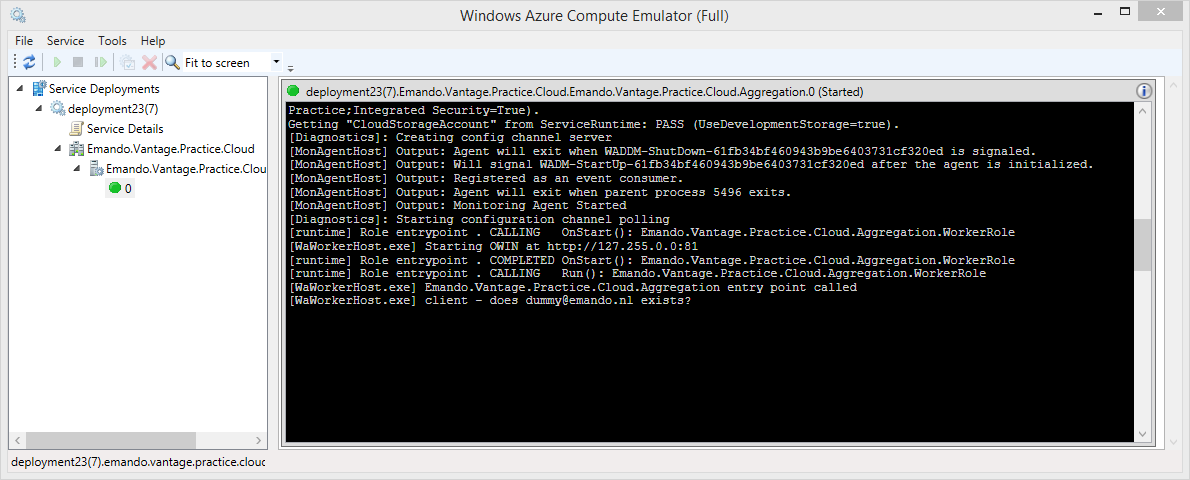
\includegraphics[height=5cm]{style/images/screenshots/IntegrationAzure}
    \label{fig:integratie-azure}
}

\subfigure[De Passing Input Console]{
    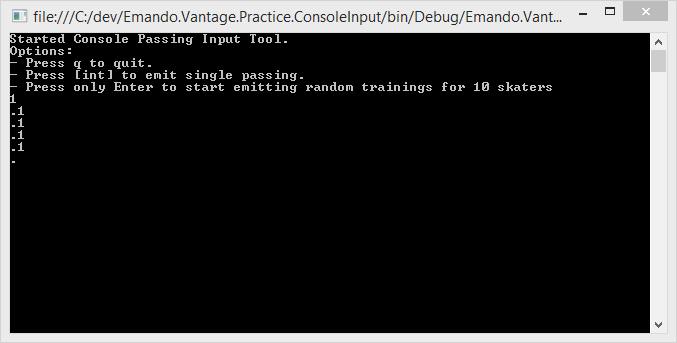
\includegraphics[height=4cm]{style/images/screenshots/IntegrationPassingInput}
    \label{fig:integratie-passing-input}
}

\subfigure[De Client Console]{
    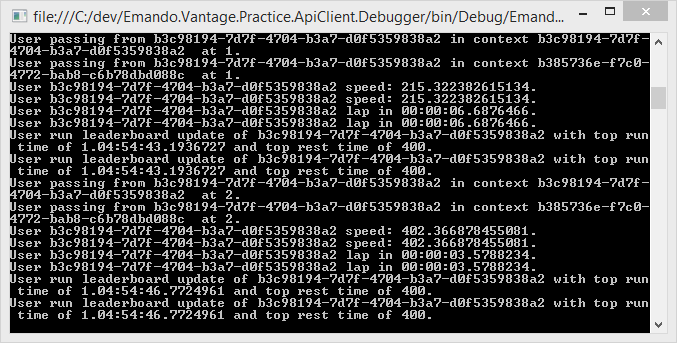
\includegraphics[height=4cm]{style/images/screenshots/IntegrationClient}
    \label{fig:integratie-client}
}
\caption{Het integratieproject voor het testen van de API Client}
\label{fig:integratie-project}
\end{figure}

Het is niet mogelijk een test van het hele platform te automatiseren op zo'n manier dat alles op een test-server draait. Voor het uitvoeren van het Azure project is een Azure Service Bus nodig die alleen in de Cloud bestaat. Azure is alleen te bereiken met de Azure SDK die alleen voor Visual Studio beschikbaar is, en dus alleen op Windows werkt, terwijl de Xamarin projecten voor iOS alleen op een MacBook kunnen opstarten. Om een speciale Mac test-server op te zetten met daarop een virtuele machine met Windows was te veel werk voor dit project, dus worden integratie-tests uitgevoerd op onze persoonlijke MacBooks, waar we deze set-up wel hebben geïnstalleerd.

% TODO: we moeten nog integratie tests schrijven in iOS.Test